\linespread{1.5}
Ondas de gravidade em um tanque d'água longo, estreito e raso, obedecem à equação de onda:
\begin{equation*}
    u_{tt} = a^2u_{xx}
\end{equation*}

sendo $a$ a velocidade de propagação da onda que é dada por $a = \sqrt{gh}$, sendo $g$ a aceleração gravitacional e $h$ a profundidade da água no tanque. Considere que o eixo $x$ é o orientado no sentido do comprimento do tanque, de modo que os extremos deste último estejam nas posições $x = 0$ e $x = L$ (o tanque tem comprimento $L$). Nessas condições, pede-se:
\begin{figure}[H]
    \centering
    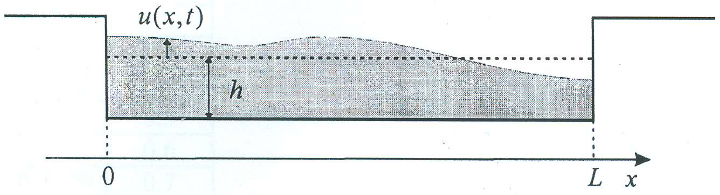
\includegraphics[width=0.5\linewidth]{fig/edp.png}
\end{figure}

\begin{itemize}
    \item[\textbf{a)}] Utilize o método da separação de variáveis para encontrar soluções particulares $u(x, t)$ da equação da onda, sujeita às condições de contorno $u_x(0, t) = 0$ e $u_x(L,t) = 0$ (A derivada parcial da solução é nula nas extremidades do tanque).
    \item[\textbf{b)}] Verifique que as soluções assim obtidas são funções periódicas do tempo. Identifique aquela solução que tem o período mais longo no tempo e faça um esboço do gráfico da mesma em função de x, para diversos valores fixos de t.
    \item[\textbf{c)}]Calcule o período da solução a que se refere o item \textbf{b)} para um tanque com comprimento de 50 m e profundidade de água de 2 m.
\end{itemize}